\begin{frame}
  \frametitle{Results for the Previous Week}

  \begin{center}
    Here are the results for last week:

    \bigskip
    
    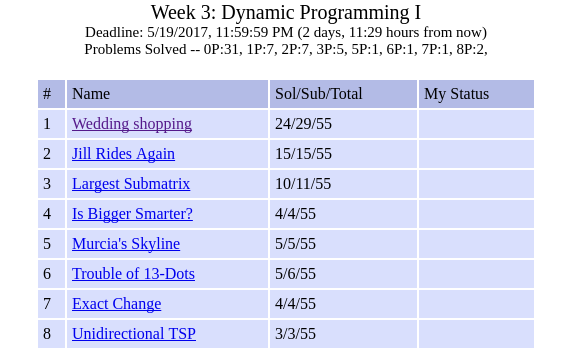
\includegraphics[width=0.8\textwidth]{img/resultsW3}

    \bigskip
    
    Great Results!
    
  \end{center}
\end{frame}

\begin{frame}
  \frametitle{Pre-class Notes (1/2) -- ICPC Dates}

  The dates for the ICPC contest this year are as follows:

  \bigskip
  
  \begin{itemize}
  \item Registration Deadline -- 06/30 (Friday)
  \item National Contest -- 07/14 (Friday)
  \end{itemize}

  \bigskip

  If you want to participate, please talk to me after class or by
  e-mail. (A team need 3 members)
\end{frame}

\begin{frame}
  \frametitle{Pre-class Notes (2/2)}

  \begin{itemize}
  \item I have moved the class {\bf Dynamic Programming II} from
    Week 4 to Week 9;

    \bigskip
    
  \item The idea is that we will use class 9 to mix different
    techniques together: (Maths, Graphs, Geometry, DP)

    \bigskip
    
  \item It will be fun :-)
  \end{itemize}  
\end{frame}

